%% ==============================================================================
%% figures_layout.tex: 独立全局图布局控制器 (Decoupled Visual Framework)
%% 将所有图画声明从正文章节中彻底抽离，实现图与正文文本解耦。
%% 正文纯文本与数学公式将自由流动，自适应无缝填充图下方留出的全部空白！
%% ==============================================================================

%% [Figure 1]: 电路图建模范式对比 (锁定第 1 页右上角，精炼图注)
\newcommand{\renderFigureIntro}{%
\begin{figure}[t]
  \centering
  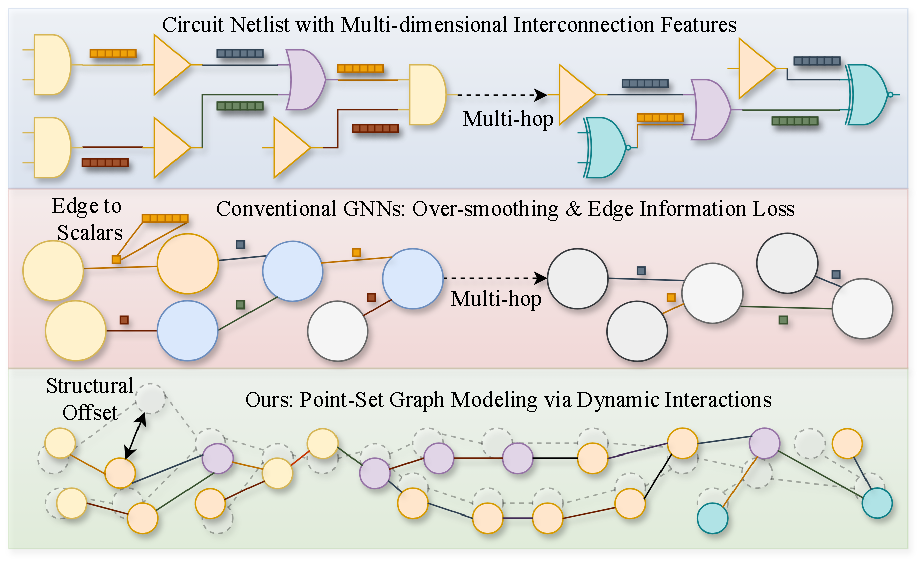
\includegraphics[width=\linewidth]{figures/intro01.pdf}
  \caption{Comparison of circuit modeling paradigms. Unlike conventional GNNs that compress edge parasitics into scalars and suffer from deep over-smoothing, our point-set dynamics preserves multi-dimensional relation vectors and drives directional coordinate offsets.}
  \label{fig:intro_paradigm}
\end{figure}%
}

%% [Figure 2]: 五阶段全局动力学演化大图 (锁定第 3 页正上方跨双栏，4 行精炼架构全景导读)
\newcommand{\renderFigureFramework}{%
\begin{figure*}[t]
  \centering
  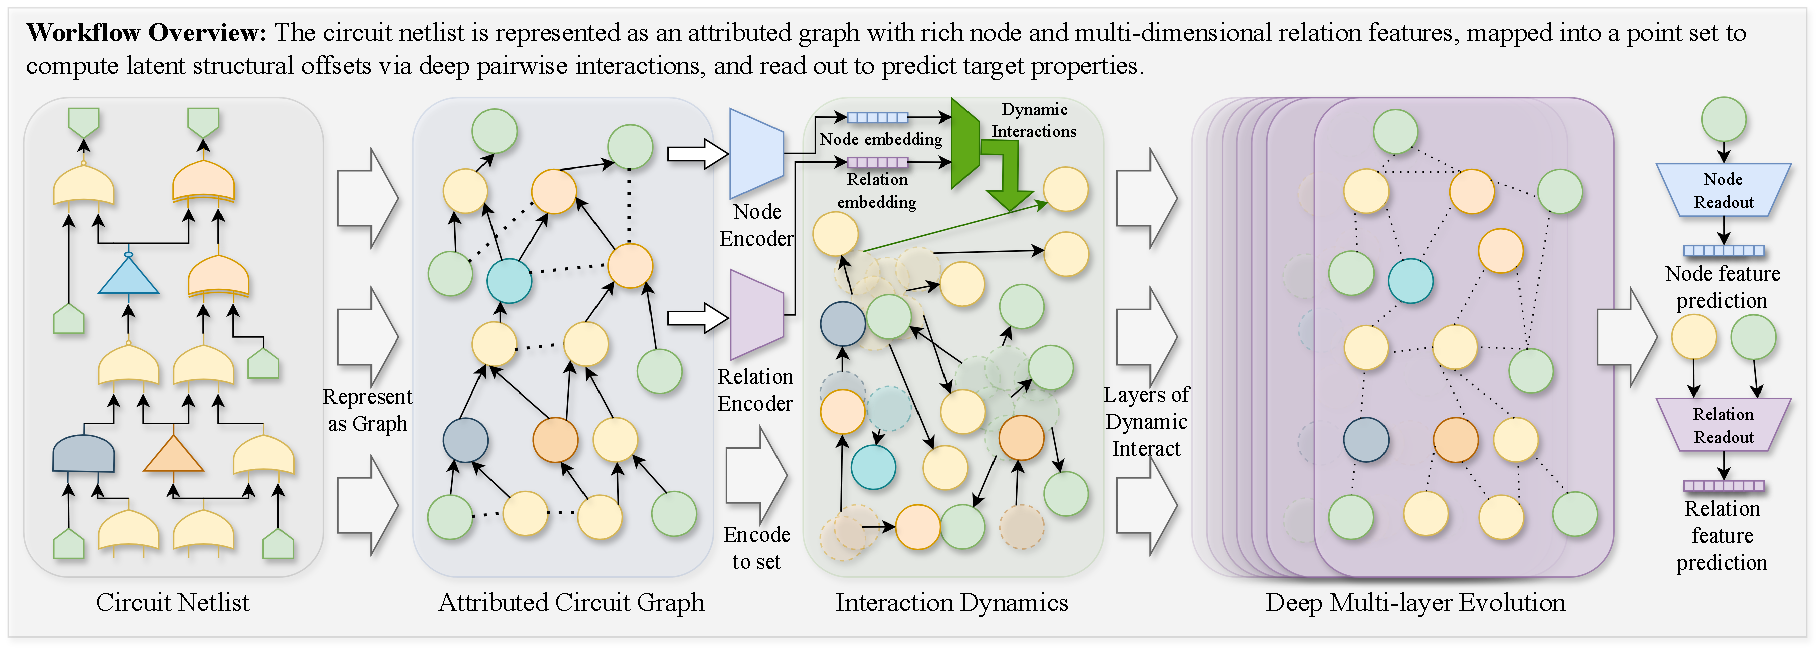
\includegraphics[width=\textwidth]{figures/method01.pdf}
  \caption{Overall framework of the point-set graph dynamics across five coordinated stages. Stage~1 extracts attributed netlists with balanced node channels and uncompressed relation vectors. Stage~2 aligns heterogeneous modalities into native latent coordinates and dense relation vectors. Stage~3 drives pairwise particle displacements via algebraic divergence and localized sibling competition. Stage~4 executes deep multi-layer additive evolution preserving non-dissipative variance across long paths. Stage~5 performs unified prior-free intrinsic readout for micro-level pins, pair-level interconnects, and macro-level PPA metrics via hierarchical virtual meter pyramids.}
  \label{fig:overall_framework}
\end{figure*}%
}

%% [Figure 3]: 局部相互作用场与同伴竞争核 (独立单栏置顶，锁定第 4 页左栏)
\newcommand{\renderFigureDynamics}{%
\begin{figure}[t]
  \centering
  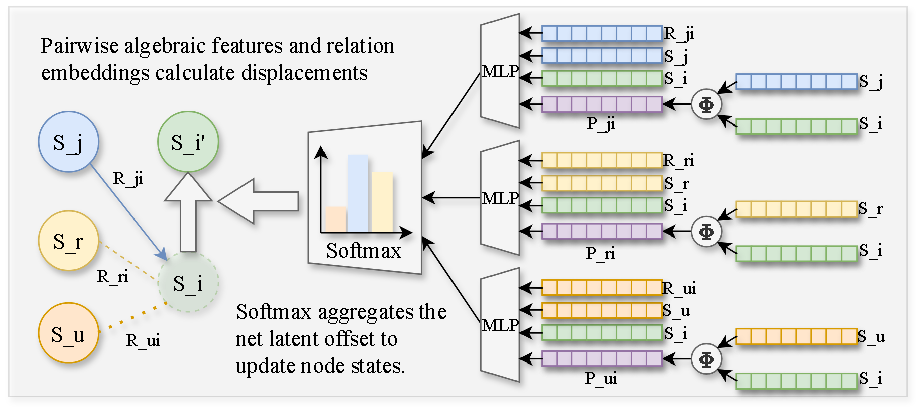
\includegraphics[width=\linewidth]{figures/method02.pdf}
  \caption{Microscopic architecture of the pairwise interaction dynamics field and localized sibling competition arbitration.}
  \label{fig:pairwise_dynamics}
\end{figure}%
}

%% [Figure 4]: 分层虚拟电表网络金字塔 (独立单栏置顶，锁定第 4 页右栏，正文自适应填补下方空白)
\newcommand{\renderFigureMeters}{%
\begin{figure}[t]
  \centering
  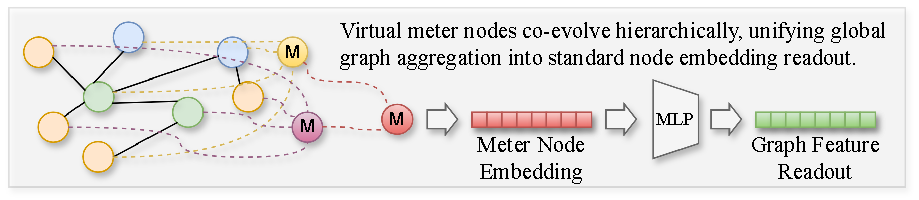
\includegraphics[width=\linewidth]{figures/method03.pdf}
  \caption{Hierarchical virtual meter network structured in a parallel reduction pyramid for unified whole-graph readout.}
  \label{fig:virtual_meter}
\end{figure}%
}
